\section{Problema III: Guardando el tesoro}

\subsection{Introducción}

Una vez pasadas todas las pruebas, Indy y el grupo de arqueólogos se encuentran en una sala llena con N tipos de tesoros de los que se sabe su valor y su peso. 
El grupo desea saquear el templo maximizando el beneficio del botín que pueden meter en sus M mochilas de capacidades diferentes.
Para decidir que tipos de tesoros tomar y en que cantidad, se pidió desarrollar un algoritmo que devuelva el valor del mejor botín y como deben estar distribuidos los tesoros en las distintas mochilas.

En las próximas secciones se usarán las siguientes notaciones para referir a distintas variables del problema:

\begin{itemize}
\item $M =$ cantidad de mochilas disponibles
\item $N =$ cantidad de tipos de tesoros
\item $K_i = $ capacidad de la mochila $i$ ($1 \leq i \leq M$)
\item $C_i = $ cantidad de tesoros del tipo $i$ ($1 \leq i \leq N$)
\item $P_i = $ peso de cada tesoro $i$ ($1 \leq i \leq \sum C_i$)
\item $V_i = $ valor de cada tesoro del tipo $i$ ($1 \leq i \leq \sum C_i$)
\end{itemize}

\subsection{Resolución del problema}
La primer propuesta tomada en cuenta fue diseñar un algoritmo que haga uso de la técnica de backtracking para resolver problema. Sin embargo, la complejidad del mismo resultó ser $O(M*(\sum_{i=0}^{M}{C_i})!)$. Esto se debía a que, por las características de la técnica usada, se probaba poner toda las combinaciones posibles de tesoros en cada mochila.

Dicha complejidad superaba en demasía la complejidad pedida por el enunciado por lo que se estudiaron las propiedades del algoritmo para implementar la mayor cantidad de podas posibles e intentar, de esta forma reducir el tiempo de ejecución.

Durante esté análisis se vio que muchos casos, llegado a cierto punto, debían recalcular subproblemas que ya habían sido calculados en otro momento y se decidió cambiar el backtracking por el uso de programación dinámica para evitar este overhead innecesario.

\subsubsection{La función recursiva}
Suponiendo que los tesoros del templo están organizados en un array de longitud $\sum C_i$, en la que cada posición del mismo contiene un único tesoro (pudiendo haber repetidos si hay mas de un tesoro de un mismo tipo), se propuso la siguiente función recursiva para calcular cual es el mejor valor posible del botín:

\begin{align*}
F(i, x_1, \dots, x_n) = \mbox{Máximo valor posible del botín con } i \mbox{ tesoros y una mochila de capacidad } x_1, \\ \mbox{una de capacidad }x_2,\dots, \mbox{y una mochila de capacidad }x_n    
\end{align*}

Sea $F^j(i) = F(i, x_1,\dots,x_{j-1}, x_j - P_{i+1},x_{j+1}\dots,x_n)$ entonces se puede escribir $F$ como:
% TODO ARREGLAR
\begin{align*} 
F(i, x_1, \dots, x_n) =
\left\{
	\begin{array}{ll}
	    0 & \mbox{si } i = 0 \lor (\forall~ 1 \leq j \leq n) ~ x_i = 0 \\
	    F(i-1, x_1, \dots, x_n) & \mbox{si } (\forall~ 1 \leq j \leq n) ~ P_i > x_j \\
	    -\infty & \mbox{si } (\exists ~ 1 \leq j \leq n) ~x_i < 0 \\
	    max\left\{\begin{array}{c}
	        F(i-1, x_1, \dots, x_M), \\
	        V_i + F^1(i-1), \\
	        \vdots\\
	        V_i + F^j(i-1) \\
	        \vdots \\
	       V_i + F^n(i-1)\\
	    \end{array}
	       \right\} & \mbox{sino} \\
	\end{array}
\right.
\end{align*}

\newpage
La función está divida en 4 casos:
\begin{itemize}
\item  \textbf{Primer caso:} No hay tesoros que poner o todas las mochilas tienen capacidad cero. En este caso no hay botín posible y el mejor valor es $0$.
\item  \textbf{Segundo caso:} El $i$-ésimo tesoro no entra en ninguna de las mochilas disponibles, entonces se debe conseguir el mejor botín sin tenerlo en cuenta.
\item \textbf{Tercer caso:} Este es un caso especial al cual solo se llega si se intenta meter un tesoro cuyo peso es mayor a la capacidad de la mochila. En la función es tomado en cuenta para que en el cuarto caso, si sucede que una mochila no puede contener el tesoro el valor sea lo mínimo posible y no afecte al resultado real de la instancia del problema
\item \textbf{Cuarto caso:} El $i$-ésimo tesoro entra en una o más mochilas. Se busca maximizar el valor del botín, por lo tanto se calcula el máximo entre el valor del botín resultante de no poner el tesoro y el máximo botín conseguido al poner el tesoro en alguna mochila.
\end{itemize}

Se debe notar que en el último caso se calculan los valores del botín resultantes de poner el tesoro en cada mochila, cada uno de estos cálculos es necesario ya que las instancias más chicas generadas al meter el tesoro en mochilas distintas son distintas.

Por último, si se desea que la función devuelva la solución al problema propuesto se la debe llamar de la siguiente forma $F\left(\sum C_i, K_1, K_2,\dots,K_M\right)$

\subsubsection{Desarrollo del algoritmo}
Al momento de implementar la función se optó por resolverla con un algoritmo bottom-up que opere sobre los valores de una matriz multidimensional.

Dicha matriz, es una matriz de M + 1 dimensiones cuyos tamaños son las capacidades de las mochilas y la cantidad de tesoros incluidos en el botín. La celda $matriz[i_1,i_2,\dots,i_{M+1}]$ representa el valor $F(i_1, i_2,\dots,i_{M+1})$.

Se ve que la matriz generada es una matriz de $\left(\sum C_i\right)\times K_1\times\dots\times K_M$ celdas

De esta forma, todos las celdas cuyos índices son de la forma $[i, 0, 0,\dots,0]$ ó $[0, x_1, x_2, \dots, x_m]$ (que corresponden al caso base de la función) son inicializadas con ceros. A partir de aquí, la matriz se recorre de manera incremental calculando los valores de cada celda a partir de los valores de las celdas calculadas anteriormente. Para aclarar esto, el algoritmo resuelve el valor de la celda $[j,j_1,\dots,j_m]$ (que corresponde al valor $F(j,j_1,\dots,j_m)$) usando los valores de las celdas $[j-1,j_1,j_2\dots,j_m],[j-1,j_1,j_2-1,\dots,j_m],\dots,[j-1,j_1,j_2,\dots,j_{m-1}-1,j_m],[j-1,j_1,j_2-1,\dots,j_{m-1},j_m - 1]$ (es decir, de cada una de las celdas superiores respecto a cada una de sus dimensiones) de acuerdo a lo indicado por la función $F$.

Una vez calculados todos los valores, solo debemos encontrar el camino desde \\ $matriz\left[\sum C_i, K_1, K_2,\dots,K_M\right]$ hasta $matriz[0,K'_1,\dots,K'_2]$ que hace posible el valor guardado en la primer posición mencionada (los valores $K'_j$ son las capacidades finales de las mochilas, es posible que el mejor botín encontrado deje, en alguna de ellas, espacio que no pueda ser llenado por ninguno de los tesoros restantes).

Para encontrar este camino se usan los siguientes criterios:
\begin{itemize}
\item Si la mejor solución encontrada para el $i$-ésimo tesoro es igual a la mejor solución encontrada para el $(i-1)$-ésimo tesoro, entonces el $i$-ésimo tesoro no pertenece al botín.
\item Si lo primero no sucede, el tesoro pertenece al botín y debe ser puesto en algún mochila. Para identificar dicha mochila se debe probar meterlo en cada una de ellas hasta encontrar la celda cuyo valor sumado al valor del $i$-ésimo tesoro sea el valor del botín completo.
\end{itemize}

\newpage
\subsection{Pseudocódigo}

Todos los algoritmos tienen acceso a \textit{tesoros} la lista de tesoros y \textit{mochilas} la lista de mochilas disponibles.

\begin{algorithm}[H]
\caption{Resolver}
\begin{algorithmic}[1]
\Procedure{Resolver}{}

  	\State	dimensions $\gets\left[\sum C_i, K_1, \dots, K_M\right]$  \Comment O(M + 1)
	\State	matrix $\gets$ MultidimensionalMatrix(dimensions);	 \Comment O($\prod$ dimensions[i])
    \State  index $\gets$ [1,0,\dots,0]  \Comment Hay M ceros O(M+1)
    
    \While{index[0] $\leq$ $\sum C_i$} \Comment Se repite $\prod$ dimensions[i] veces
		\State	matrix.set(index, maxValue(matrix, index)) \Comment Setear la celda index de la  matriz al 
		\State  \Comment valor correspondiente O(M)
		\State	index $\gets$ nextIndex(matrix, index) \Comment O(1)
	\EndWhile
	\State	index $\gets$ previousIndex(matrix,index);
	\State	lootValue $\gets$ matrix.get(index);
	
	\While{index[0] $>$ 0}	 \Comment Se repite $\prod$ dimensions[i] veces
		\State	m $\gets$ whereToPutTreasure(matrix, index); \Comment Conseguir la mochila donde poner el tesoro O(m)
	    \If{m $<$ 0}
			\State	index[0] $\gets$ index[0] - 1; \Comment No poner el tesoro
        \Else	
			\State agregar(tesoros[index[0]], mochilas[m]) \Comment Agregar el tesoro a la $m$-ésima mochila. O(1)
			\State	index[0] $\gets$ index[0] - 1; \Comment Con estas dos líneas se mueve a la celda que representa
			\State	index[m] $\gets$ index[m] - peso(tesoros[index[0]]) \Comment la instancia generada al poner el 
			\State \Comment tesoro en la mochila
		\EndIf
    \EndWhile
\EndProcedure
\end{algorithmic}
\end{algorithm}

El paso en el que se rellenan con ceros las posiciones indicadas por el caso base de la función recursiva es omitido pues se asume que todas los valores de la matriz son inicializados en cero.

\begin{algorithm}[H]
\caption{maxValue}
\begin{algorithmic}
 
  \Procedure{maxValue}{MultidimensionalMatrix matrix, Integer[] index} $\to $ \texttt{Integer}
 		
 		\State auxIndex $\gets$ index
		\State auxIndex[0] $\gets$ auxIndex[0] - 1 \Comment Esta es la celda que corresponde a no poner el tesoro index[0]

        \State maxValue $\gets$ matrix.get(auxIndex) \Comment El valor del botín sin el tesoro
        \For {m = 1 to dimensiones(matrix)}  \Comment Se repite M veces
			\If{index[m] $>=$ peso(tesoros[index[0]])} \Comment Si la capacidad de la mochila $m$ es suficiente
			\State	auxIndex[m] $\gets$ index[m] - peso(tesoros[index[0]]); \Comment Poner el tesoro en la mochila $m$ O(1)
			\State	newValue $\gets$  valor(tesoro[index[0]]) + matrix.get(auxIndex); \Comment Conseguir el valor del botín \If{newValue $>$ maxValue} \Comment Si el valor que se consigue es mejor que el de los otros intentos
			\State maxValue $\gets$ newValue; \Comment se setea como maximo
			\EndIf
			
			\State auxIndex[m] $\gets$ auxIndex[m] + peso(tesoros[index[0]]) 	\Comment Sacar el tesoro de la mochila
			\EndIf
		\EndFor
    	\State Devuelvo maxValue
	\EndProcedure
 \end{algorithmic}
\end{algorithm}

\begin{algorithm}[H]
\caption{whereToPutTreasure}
\begin{algorithmic}[1]
  \Procedure{whereToPutTreasure}{MultidimensionalMatrix matrix, Integer[] index} $\to $ \texttt{Integer}

    \State auxIndex $\gets$ index 
    \State auxIndex[0] $\gets$ index[0]-1 
	\State actualValue $\gets$ matrix.get(index)
	\State maxValue $\gets$ matrix.get(auxIndex);
	
	\If{maxValue == actualValue}    \Comment Si el botín con el tesoro y el botín sin el tesoro
	    	\State Devolver -1  \Comment  tienen el mismo valor entonces omitirlo
	\EndIf
		
	\State	maxValue $\gets$ 0  \Comment Setear el valor maximo a cero

    \For {m = 1 to dimensiones(matrix)}  \Comment Se repite M veces
		\If{index[m] $\geq$ peso(tesoros[index[0]])} 
		\State	auxIndex[m] $\gets$ index[m] - peso(tesoros[index[0]])
		\State	newValue $\gets$  valor(tesoro[index[0]]) + matrix.get(auxIndex);

    	\If{newValue == actualValue)}	
            \State	whereToPut $\gets$ m 
            \State	maxValue $\gets$ newValue
		\EndIf
		\State	auxIndex[m] $\gets$ index[m] 
    \EndIf
	\EndFor
		
	\State	Devolver whereToPut
\EndProcedure
\end{algorithmic}
\end{algorithm}

Se puede ver que las funciones whereToPutTreasure y maxValues son similares. En ambas funciones se checkean los valores de las soluciones anteriores para decidir, en una, cual es el máximo valor de botín posible y, en la otra, en que mochila debo ubicar cierto tesoro para conseguir el botín que corresponde al valor ubicado en la celda pasada por parámetro.

\subsection{Correctitud}
El algoritmo propuesto puede ser dividido en partes:
\begin{enumerate}
    \item El cálculo del valor del mejor botín
    \item Calcular los tesoros que pertenecen a dicho botín y en que mochila deben ser guardados.
\end{enumerate}

Como se explicó en la sección 4.3.3, la primer parte del algoritmo corresponde al cálculo de la función $F$ para sus distintos parámetros de entrada.

\subsubsection{Primer parte}
Por inducción, se puede ver que el primer paso es correcto:

\textbf{Casos Base:}

\begin{itemize}
\item $\sum C_i = 0$:
    
    Al no haber tesoros que poner en las mochilas, no hay botín posible, por lo tanto no hay valor positivo para el mismo.
    
    En la implementación del algoritmo, la matriz es inicializada con todos sus valores en $0$ pero no es modificada por el while correspondiente a esta parte del algoritmo. Por lo que $lootValue = 0$.
    
\item $K_i = 0 ~\forall~ 1\leq i \leq M$

    Todas las mochilas tienen capacidad cero y como el peso de cualquier tesoro es mayor a cero, entonces no existe un tesoro que entre en ninguna de ellas. Esto quiere decir que no hay botín posible, entonces, no hay valor positivo para el mismo.
    
    Otra vez, se ve que el algoritmo respeta este caso, las iteraciones son realizadas, pero al momento de calcular el máximo valor del botín, se toma el valor de la solución anterior (que es 0) y se itera sobre todas las mochilas. Sin embargo, al tener todas ellas capacidad cero, en ninguna iteración se accede al if que remplaza el valor máximo por uno distinto. Luego, el resultado de esta operación termina siendo cero.
    
    En un primer paso se calcula el valor de poner cero tesoros en las mochilas (este es el caso anterior) entonces este valor es cero. Luego, se trata de poner un tesoro pero, por las operaciones que realiza el algoritmo este valor será el mismo que el de la solución anterior entonces el mejor botín con un tesoro tiene valor 0.
    
    En el n-ésimo paso, la solución será la misma que en el (n-1)-ésimo que, como se explicó, es 0. Esto implicaría que en el n-ésimo paso la solución seguirá siendo 0.
    
    Por último, habiendo demostrado esto, se concluye que en último valor calculado \\ $\left(M\left[\sum C_i, K_1, \dots, K_M\right]\right)$ es 0.
\end{itemize}

\textbf{Paso inductivo:}

    Sea la hipótesis inductiva que el algoritmo es correcto para todas las instancias tal que hay $i-1$ tesoros, se puede deducir la correctitud del $i$-ésimo:
    
    \begin{align*}
    F(i, x_1,\dots,x_M) &= 	max\left\{ F(i-1, x_1, \dots, x_M), V_i + F^1(i-1), \dots,
	        V_i + F^j(i-1), \dots, V_i + F^n(i-1)\right\} \\ &= max\left\{F(i-1, x_1,
	        \dots, x_M), V_i + max\left\{F^1(i-1), \dots, F^j(i-1), \dots, F^n(i-1)\right\}\right\}    
    \end{align*}
    
    Por la hipótesis inductiva, sabemos que $ F(i-1, x_1, \dots, x_M)$, $F^1(i-1),\dots, F^n(i-1)$ son correctas.
    
    Se puede ver que la función toma el máximo entre todas las posibilidades dados $i$ tesoros con la configuración de mochilas dadas.
    
    La función devuelve el máximo valor de entre no agregar el tesoro y agregarlo a alguna mochila. Por \textit{HI}, el primer valor es correcto, veamos que el segundo valor lo es:
    
    El segundo valor toma el máximo botín que se puede obtener si fuese que se reserva un lugar para el $i$ ésimo tesoro en alguna mochila.
    Si $F^j(i-1)$ corresponde al mejor botín posible con esta característica, entonces el segundo valor es de la forma $V_i + F^j(i-1)$. Y si este no fuera el mejor valor posible, entonces existiría otro botin con valor $V_i + F^k(i-1)$, en este caso resultaria que $F^k(i-1) > F^j(i-1)$ pero esto sería absurdo por que $F^j(i-1)$ era el máximo.
    
    El algoritmo propuesto realiza esta operación de la manera clásica, asigna un valor inicial a la variable $maxValue$ ($ F(i-1, x_1, \dots, x_M)$) y luego itera sobre las posiciones de la matriz que corresponden a intentar meter el botín en las distintas mochilas disponibles. Cuando se ve que, al ubicar el tesoro en cierta mochila, se consigue un valor mayor a $maxValue$, este es reemplazado por el nuevo valor encontrado.
    
    Al finalizar las iteraciones, $maxValue$ contendrá el máximo valor posible del botín.
    
\subsubsection{Segunda parte}
Este paso consiste en reproducir las selecciones de los máximos elegidos en la sección anterior. Para esto, se checkean uno a uno los valores de cada instancia más chica del problema llamada en $F$.

La primer celda checkeada corresponde a la solución en la que el tesoro no es agregado y si el valor de esta solución y la solución que se esta buscando es igual, entonces el tesoro es omitido.
Al resto de los valores se le suma el valor del tesoro que se intenta agregar, si el resultado es igual al valor de la celda que se está analizando entonces el tesoro se agrega a la mochila que corresponde al índice desplazado. 
Este desplazamiento corresponde al valor máximo elegido por la función $F$ y estas operaciones se realizan de forma iterativa hasta que la celda analizada represente alguno de los casos bases de $F$.

Cuando el algoritmo finaliza, las mochilas contienen la sucesión de tesoros necesaria para poder lograr un botín de valor óptimo.

\subsection{Complejidad del algoritmo}

Al momento de calcular la complejidad de los algoritmos propuestos se asumió que el acceso a una posición de la matriz multidimensional es $O(1)$. 

\subsubsection{maxValue y whereToPut}
En los algoritmos $maxValue$ y $whereToPutTreasure$, los $for$ realizan $M$ iteraciones en las cuales se accede y/o modifica la matriz y distintas variables enteras, cada una de estas operaciones es $O(1)$. En ambos casos los condicionales de los $if$ dentro del $for$ hacen comparaciones de enteros por lo que estas comparaciones se realizan en $O(1)$.
Las asignaciones realizadas fuera del $for$ son realizadas en $O(1)$, salvo la variable $auxIndex$ que es inicializada en $O(M+1)$.

Luego ambos algoritmos son de complejidad $O(M + M + 1) \subset O(M)$.

\subsubsection{resolver}
En el algoritmo $resolver$, se crean 2 arrays (\texttt{dimensions} e \texttt{index}) de $M+1$ elementos cada uno ($O(M+1)$), luego se crea la matriz multidimensional que es $O\left(\prod\texttt{dimensions}[i]\right)$ y luego se ejecutan los dos $while$. 

Con el primer $while$ se rellena cada posición de la matriz con el valor correspondiente, esto es hacer $\prod\texttt{dimensions}[i]$ iteraciones. En cada iteración se debe setear la celda correspondiente usando la función $maxValue$ ($O(M)$) y luego se aumenta el indice en 1 ($O(1)$). Entonces el $while$ completo tiene complejidad $O\left(M*\prod\texttt{dimensions}[i]\right)$

En el segundo, en peor caso, debemos volver a recorrer cada celda de la matriz por lo que se realizan la misma cantidad de iteraciones. En cada iteración se realiza una llamada a $whereToPut$ ($O(M)$) y a luego se calcula el proximo indice en $O(1)$, además, si es necesario, se agrega a una mochila un tesoro.

Las mochilas pueden ser vistas como listas enlazadas, por lo que agregarles un elemento es $O(1)$.

Por lo tanto el segundo while tiene la misma complejidad que el primero.

El algoritmo completo tiene complejidad 

$$O\left(M + 1 + M*\prod\texttt{dimensions}[i] + M*\prod\texttt{dimensions}[i]\right) \subset O\left(M*\prod\texttt{dimensions}[i]\right)$$

Ahora, \texttt{dimension[0]} es la cantidad de tesoros en la sala, es decir $\sum_{i=1}^N C_i$, entonces:

$$ M*\prod_{i=0}^M\texttt{dimensions}[i] = M*\left(\sum_{i=1}^N C_i\right)*\prod_{i=1}^M\texttt{dimensions}[i]$$

Y cada uno de los indices siguientes, corresponden a los pesos de los mochilas, es decir $indice[i] = K_i$ para $1 \leq i \leq M$ y vale:

$$M*\left(\sum C_i\right)*\prod_{i=1}^M\texttt{dimensions}[i] = M*\left(\sum C_i\right)*\prod_{i=1}^M K_i$$

Luego el algoritmo completo es de complejidad $O(M*\left(\sum_{i=1}^N C_i\right)*\prod_{i=1}^M K_i)$, solo falta ver que dicha complejidad es menor a la requerida por el enunciado, es decir se necesita comprobar que:


\[
O\left(M*\left(\prod_{i=1}^{M}{K_i}\right)*\left(\sum_{i=1}^{N}{C_i}\right)\right) \subset O\left(\left(\sum_{i=1}^{M}{K_i}\right)^{M}*\left(\sum_{i=1}^{N}{C_i}\right)\right)
\]

Para ver que esto es cierto basta con probar la siguiente desigualdad:

\[
M*\left(\prod_{i=1}^{M}{K_i}\right)*\left(\sum_{i=1}^{M}{C_i}\right) \leq \left(\sum_{i=1}^{M}{K_i}\right)^{M}*\left(\sum_{i=1}^{N}{C_i}\right)
\]

Como $\sum_{i=1}^{N}{C_i} \neq 0$ :

\[
M*\prod_{i=1}^{M}{K_i} \leq \left(\sum_{i=1}^{N}{K_i}\right)^{M}
\]

Por la fórmiula del coeficiente multinomial se sabe que:

\begin{align*}
\left(\sum_{i=1}^{M}{K_i}\right)^{M} =  \sum_{J_1+...+J_M=M}\binom{M}{ J_1,...,J_M}*\prod_{t=1}^{M}{K_i}^{J_t} = \\
M * \prod_{i=1}^M K_i + 
\sum_{ J_1,\dots,J_M : J_1 + \dots + J_M = M \land  \lnot (\forall 1 \leq i \leq M) J_i = 1}\binom{M}{ J_1,...,J_M}*\prod_{t=1}^{M}{K_i}^{J_t}
\end{align*}

El primer término mostrado en la última igualdad surge de elegir todos los exponentes iguales a 1. Por esta razón se agrega la condición $\lnot (\forall 1 \leq i \leq M) J_i = 1$ al segundo término.

En la inecuación, entonces se remplaza:

\[
M*\left(\prod_{i=1}^{M}{K_i}\right) \leq M * \prod_{i=1}^M K_i + 
\sum_{ J_1,\dots,J_M : J_1 + \dots + J_M = M \land  \lnot (\forall 1 \leq i \leq M) J_i = 1}\binom{M}{ J_1,...,J_M}*\prod_{t=1}^{M}{K_i}^{J_t}
\]

\[
0\leq \sum_{ J_1,\dots,J_M : J_1 + \dots + J_M = M \land  \lnot (\forall 1 \leq i \leq M) J_i = 1}\binom{M}{ J_1,...,J_M}*\prod_{t=1}^{M}{K_i}^{J_t}
\]


Y como todos los elementos de esta sumatoria son enteros positivos (por ser todos los $K_i$ positivos), queda demostrado que la complejidad que proponemos es menor a la pedida por el enunciado.

\subsection{Experimentación}
Para los experimentos se decidió analizar instancias se varían los tamaños de las mochilas y la cantidad de tesoros por separado. En ambos experimentos, las variaciones se prueban para 1, 2 y 3 mochilas.

En el primero de los casos, se fijó el tamaño de las mochilas en 50 unidades cada una y se generaron instancias de problemas con cantidades de tesoros variante entre 1 y 100. El precio y valor de cada uno de los tesoros fue generado aleatoriamente entre los valores 1 y 100.

Se debe notar que los valores y pesos de los tesoros no influyen en la complejidad del algoritmo por lo que no se consideró necesario evaluar instancias con valores demasiados granes.

Los resultados obtenidos se muestran en los siguiente gráficos:
\begin{figure}[H]
    \centering
    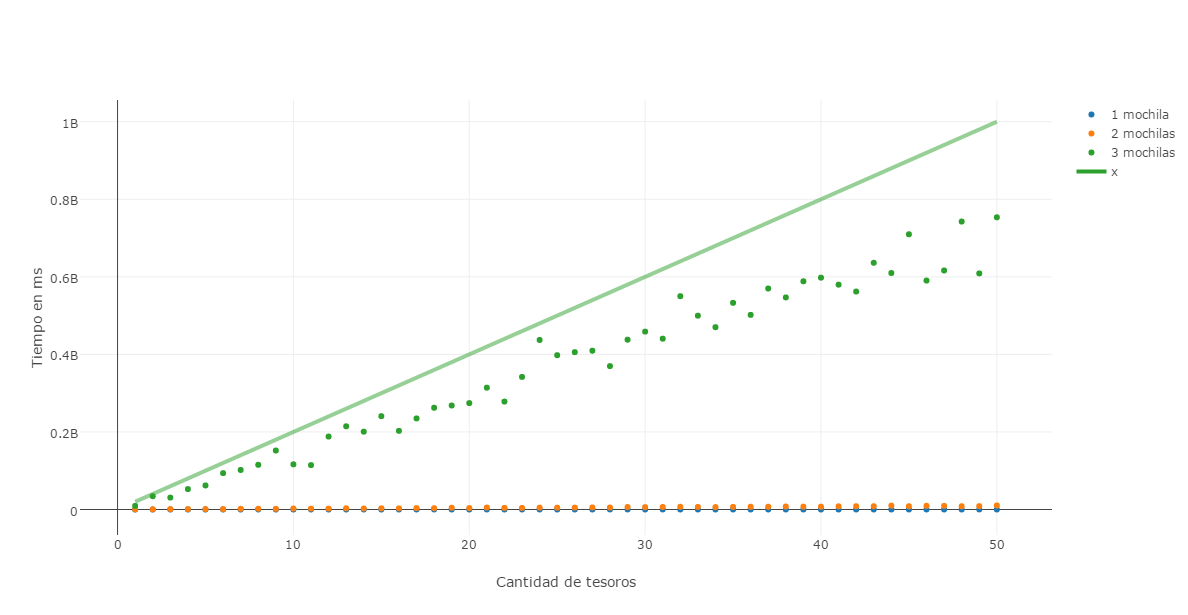
\includegraphics[width=\textwidth]{./imagenes/3-1.png}
\end{figure}

Se puede ver que para los 3 casos probados el crecimiento temporal es lineal, lo que corresponde con la complejidad teórica calculada cuando la cantidad de mochilas y sus capacidades son tomadas como constantes. Y además, se nota que al aumentar la cantidad de mochilas los tiempos para instancias con la misma cantidad de tesoros incrementan notablemente debido a que la constante se ve afectada exponencialmente por la cantidad de mochilas.

$$O\left(\left(\sum_{i=1}^{1}{50}\right)^{1}*\left(\sum_{i=1}^{N}{C_i}\right)\right) = O\left(\sum_{i=1}^{N}{C_i}\right) = 
O\left(X\right)$$


$$
O\left(\left(\sum_{i=1}^{2}{50}\right)^{2}*\left(\sum_{i=1}^{N}{C_i}\right)\right) = O\left(\sum_{i=1}^{N}{C_i}\right) = O\left(X\right)$$

$$O\left(\left(\sum_{i=1}^{3}{50}\right)^{3}*\left(\sum_{i=1}^{N}{C_i}\right)\right) = O\left(\sum_{i=1}^{N}{C_i}\right) = O\left(X\right)$$

En el siguiente, se ha realizado un experimento similar anterior diferenciándose de que todas las instancias los tesoros van a ser los mismos y se varían las capacidades de las mochilas. 

Los tesoros elegidos fueron:

\begin{tabular}{ c c c }
    Cantidad & Peso & Valor \\
    1 & 30 & 14 \\
    3 & 35 & 10 \\
    4 & 40 & 30 \\
    2 & 45 & 4 \\
    1 & 50 & 20 \\
    5 & 50 & 60 \\
\end{tabular}
 
						

En este caso, el polinomio que acota temporalmente a los tiempos calculados está dado por la cantidad de mochilas. En el siguiente gráfico se observa que para 1 mochila, los tiempos se incrementan de forma lineal, mientras que en las instancias de 2 mochilas su aumento es cuadrático y en las de 3 mochilas es cúbico.

\begin{figure}[H]
    \centering
    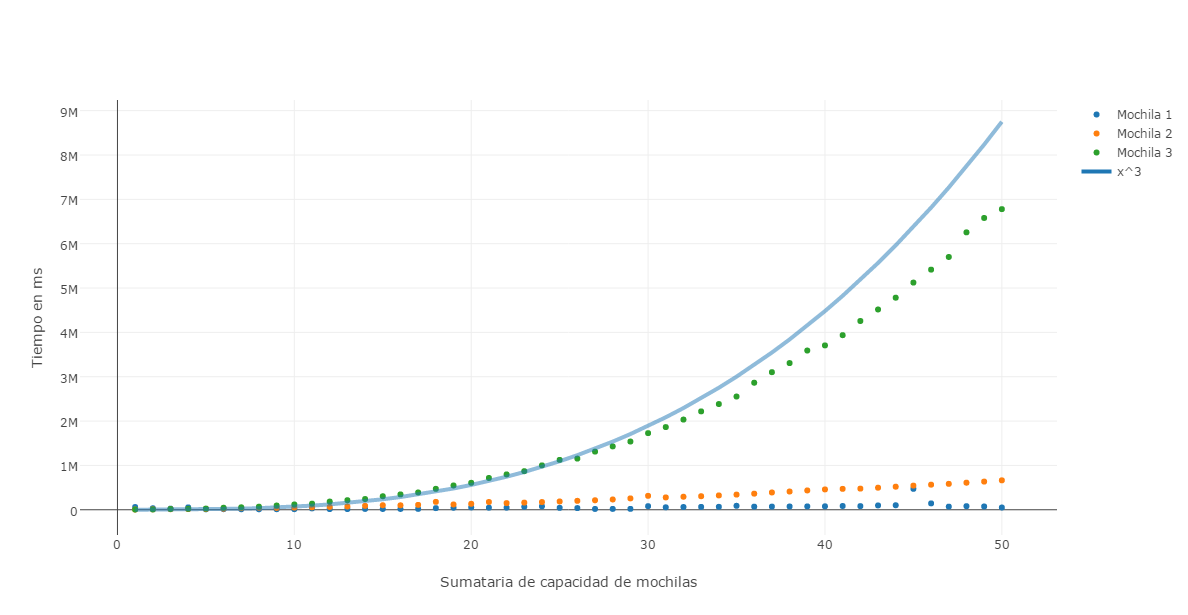
\includegraphics[width=\textwidth]{./imagenes/3-2.png}

\end{figure}

De esta forma se corrobora que la complejidad se cumpla, ya que la complejidad experimental de cada caso termina siendo:
Sea $K_i$ al peso de la i-ésima mochila:

$$O\left(\left(\sum_{i=1}^{1}{K_i}\right)^{1}*\left(\sum_{i=1}^{6}{C_i}\right)\right) = O\left(\left(\sum_{i=1}^{1}{K_i}\right)^{1}*\left(16\right)\right) = O\left(K_1\right)$$

$$O\left(\left(\sum_{i=1}^{2}{K_i}\right)^{2}*\left(\sum_{i=1}^{6}{C_i}\right)\right) = O\left(\left(\sum_{i=1}^{2}{K_i}\right)^{2}*16\right) = O\left(\left(\sum_{i=1}^{2}{K_i}\right)^{2}\right)$$

$$O\left(\left(\sum_{i=1}^{3}{K_i}\right)^{3}*\left(\sum_{i=1}^{6}{C_i}\right)\right) = O\left(\left(\sum_{i=1}^{3}{K_i}\right)^{3}*16\right) = O\left(\left(\sum_{i=1}^{3}{K_i}\right)^{3}\right) $$
